\chapter{Deep Neural Network Toolkit} 
\label{chap:toolkit}
%%%%%%%%%%%%%%%%%%%%%%%%%%%%%%%%%%%%%%%%%%%%%%%%%%%%%%%%%%%%%%%%%%%%%%%%%%%%%%%%%%%%%%%%%%%%%%%%%%%%%%%%%%%%%%%%%%%%%%%%%
\section{Introduction}
Deep Neural Network is the current trend
in machine learning. Deep Neural networks can be best implemented using the modular, object-oriented approach. 

Even though there are many tool-kits, these toolkit lacks simplicity. Moreover with recent growth of GPU programming has pave the way for fast implementation of DNN. \textit{Python-DNN} was developed with modularity, and speed in mind.

\section{Python-DNN}
\textit{Python DNN} is a lightweight deep learning toolkit developed in Python, which can run on both GPU and CPU. It makes use of \emph{theano} which allows optimisation and evaluation of mathematical expressions involving multi-dimensional arrays efficiently \cite{bergstra2010theano}.

\subsection{Existing Tool-kit/libraries}
There are many Tool-kit and libraries has been developed for Deep Neural Network. Some of them are following: 
\begin{itemize}
\item \href{http://kaldi.sourceforge.net/}{Kaldi} Speech Recognition tool-kit
\item \href{https://github.com/rasmusbergpalm/DeepLearnToolbox}{DeepLearnToolbox}, A toolkit for \textit{Matlab \& Octave}
\item \href{http://cs.stanford.edu/people/karpathy/convnetjs/}{convnetjs}, a JavaScript based library
\item \href{https://radimrehurek.com/gensim}{Gensim}, a tool-kit for NLP
\end{itemize}

There are many issues with these existing tool-kits. Major one is most of them are domain specific. Since Deep Neural Network is computationally heavy, there are fast implementation of DNN which make use of GPU. But these tool-kits work only with GPU. None of tool-kits can work seamlessly on both GPU and Multicore CPUs. 

We built a tool-kit to overcome this problem, which can also be used as a stand alone library


\subsection{Supported Models}
\label{sec:python-dnnModels}
\textit{Python DNN}  has support  for Deep Belief Network (DBN) \cite{hinton2002training} (uses Restricted Boltzmann machine(RBM)), Stacked Denoising Auto-encoders (SdA) \cite{vincent2010stacked} and Convolutional Neural Network (CNN) \cite{lecun1998gradient} (both 2D-CNN and 3D-CNN). \textit{Python-dnn} is developed in such a way that it can be easily extended to support other models in the future.

\subsection{Architecture}

\begin{figure}[ht]
\centering
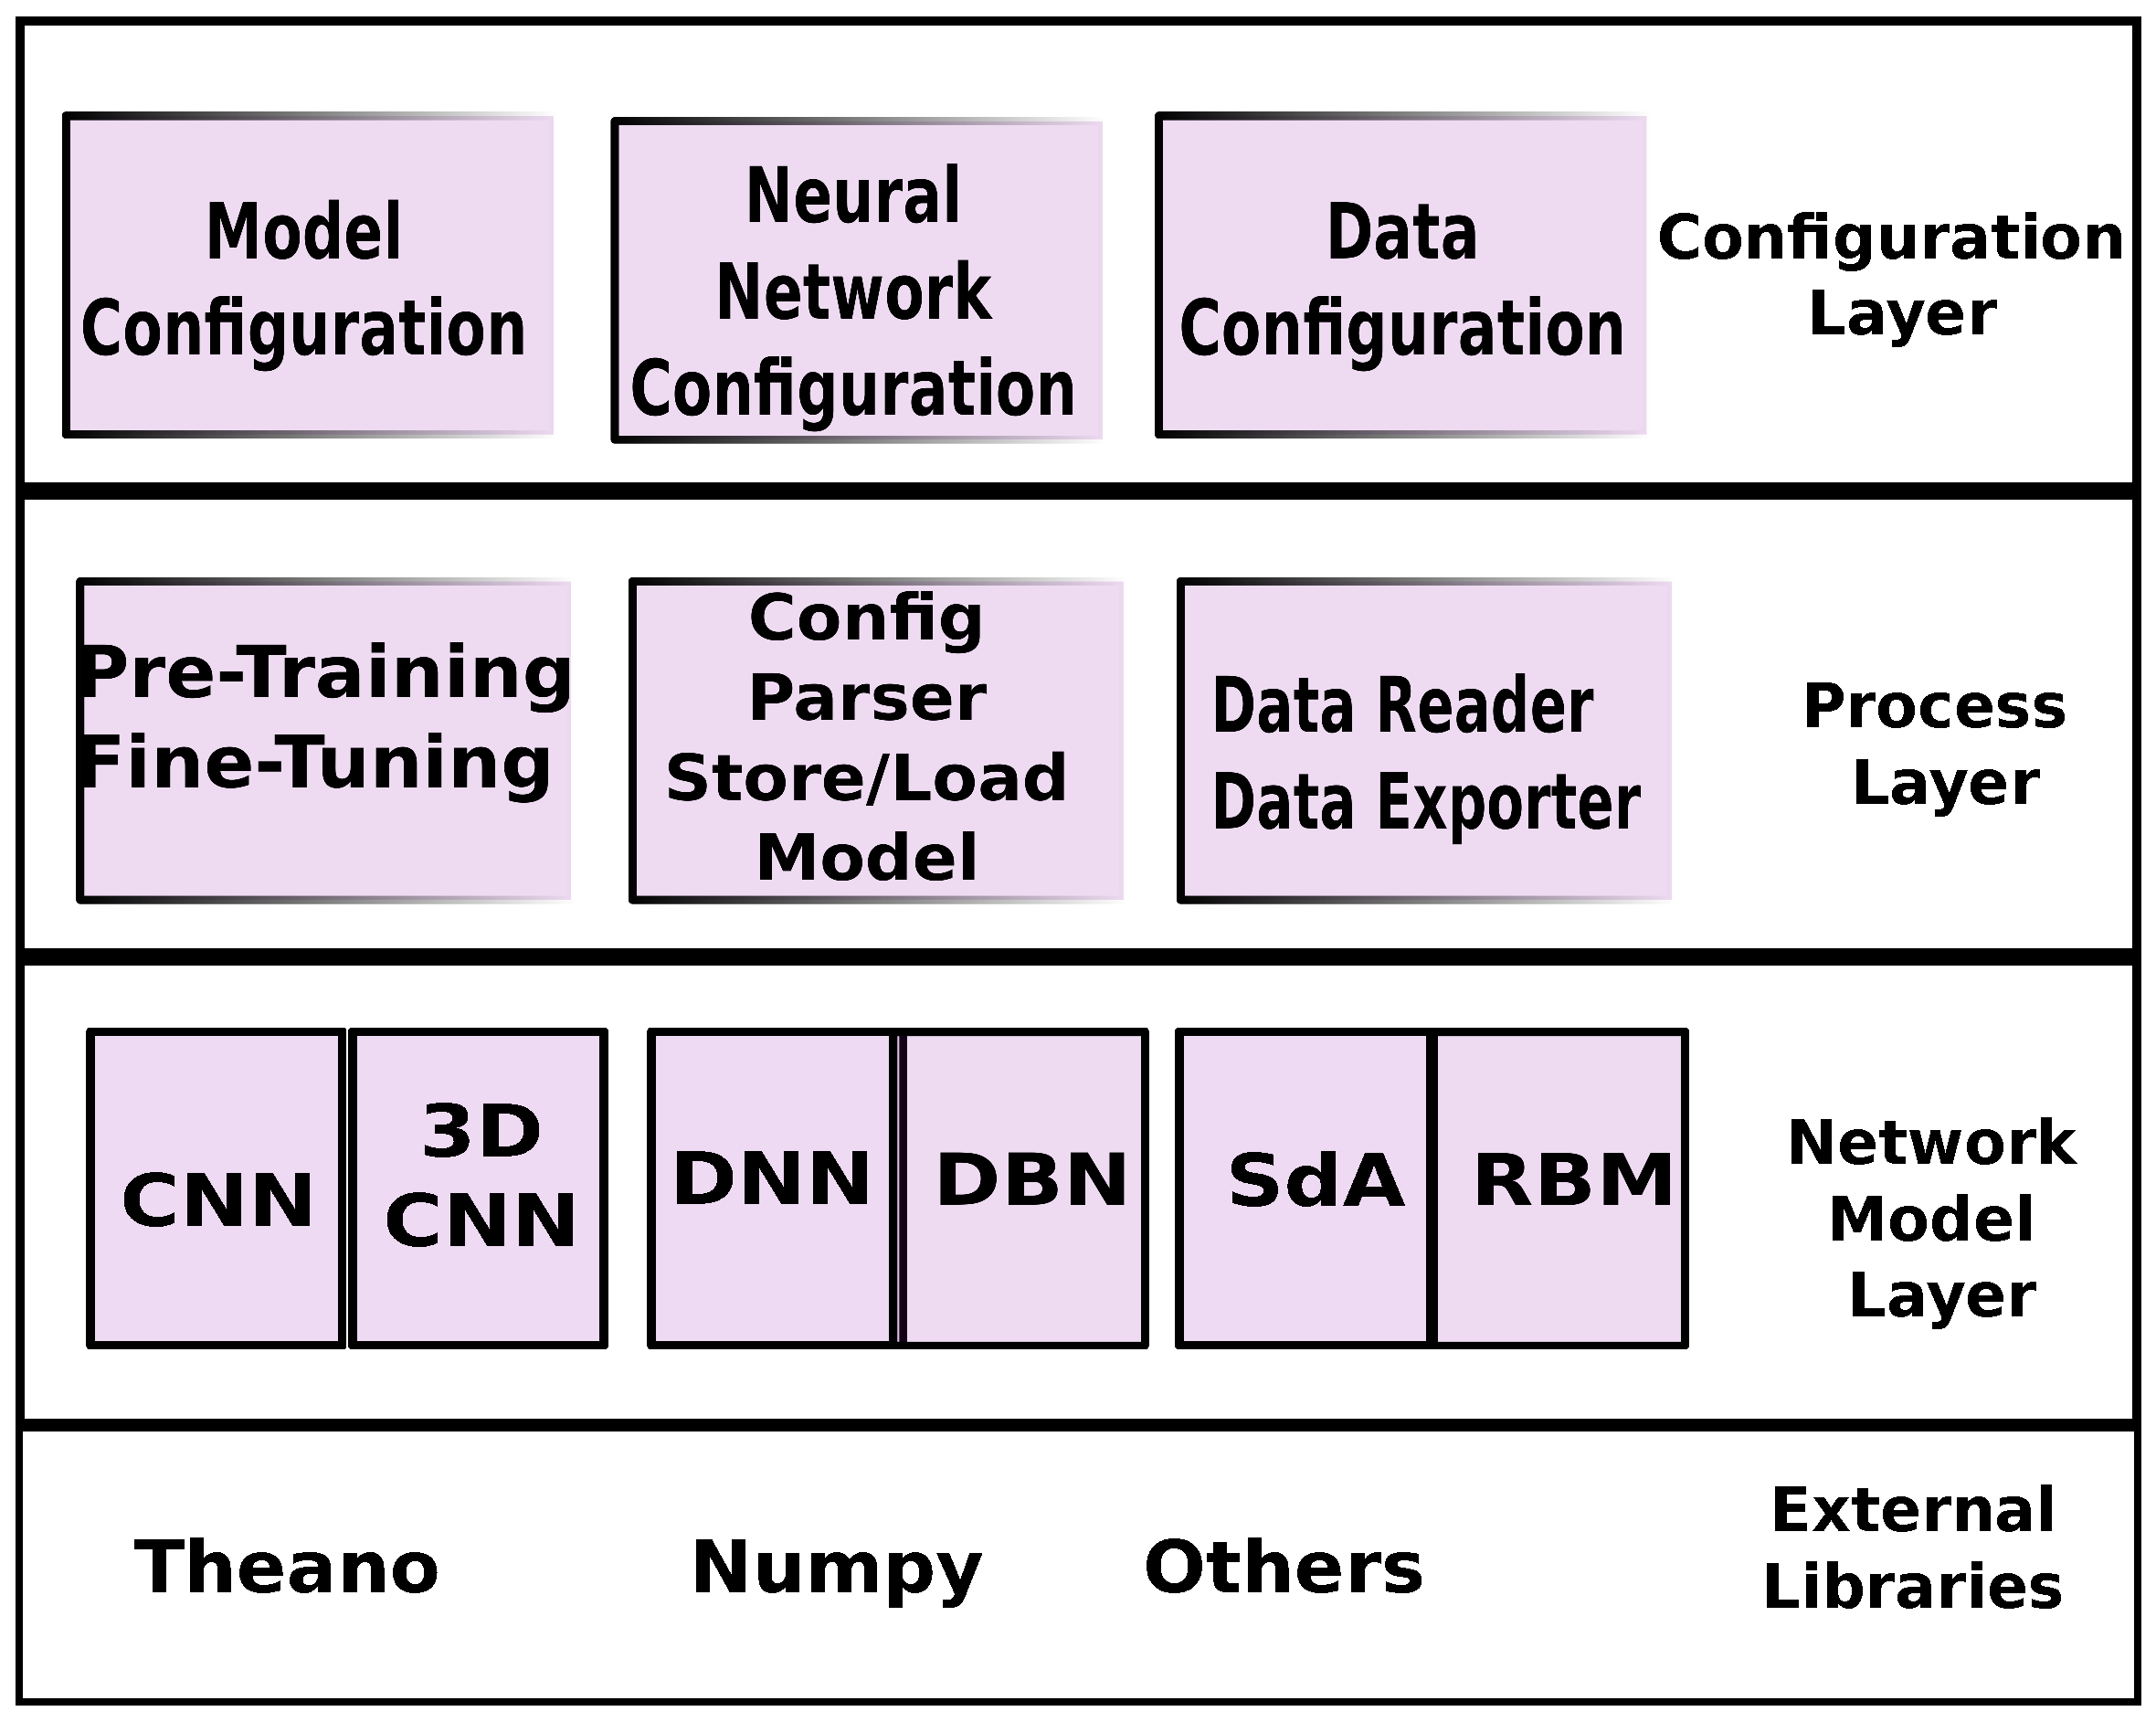
\includegraphics[width=0.7\textwidth]{./imgs/Python-DNNArch.eps}
\caption{Architecture of Python-DNN}
\label{fig:pydnn-arch}
\end{figure}

\textit{Python-DNN} uses \emph{theano} library, which provides an efficient platform for running in both CPU and GPU architectures. Architecture of our indigenous toolkit is shown on \ref{fig:pydnn-arch}. 

\noindent The tool-kit can be partitioned into 4 abstract layers:
\begin{itemize}
\item The \textit{external libraries} that includes all the dependent libraries
\item \textit{Network model layer} contain different supervised and unsupervised models.
\item The different operation on the different models is performed in \textit{processing layer}
\item The \textit{configuration layer} which specify all details of the input and model to lower layers.
\end{itemize}

Details of configuration in given in Appendix \ref{app:pythondnn}

\subsection{Salient Features}
\label{sec:python-dnnFeatures}
\begin{itemize}
\item Easy configuration of the models, configurations
are organised in JSON format and  hence make it legible to humans.
\item Run efficiently in CPU and GPU architectures.
\item Able to load the pre-trained model and dump the trained model.
\item Different types of Data Reader and Data Exporter.
\item Can be used as a standalone application as well as a standard  library.
\item Released in Apache Software License(version 2).\\
\end{itemize}

\section{Summary}
\textit{Python DNN} is a indigenous deep neural network toolkit which is easy to configure and able to make use of both GPU and CPU architectures. The toolkit is publicly hosted in github\footnote{Public repository of \textit{Python-DNN} : (\url{https://github. com/IITM-DONLAB/python-dnn})}

Further details about the the toolkit installation, configuration and its usage is explained in Appendix \ref{app:pythondnn}
%%%%%%%%%%%%%%%%%%%%%%%%%%%%%%%%%%%%%%%%%%%%%%%%%%%%%%%%%%%%%%%%%%%%%%%%%%%%%%%%%%%%%%%%%%%%%%%%%%%%%%%%%%%%%%%%%%%%%%%%
